
%
%  $Description: Author guidelines and sample document in LaTeX 2.09$
%
%  $Author: ienne $
%  $Date: 1995/09/15 15:20:59 $
%  $Revision: 1.4 $
%

\documentclass[times, 10pt,twocolumn]{article}
\usepackage{latex8}
\usepackage{times}
\usepackage{hyperref}
\usepackage{graphicx}

%\documentstyle[times,art10,twocolumn,latex8]{article}

%-------------------------------------------------------------------------
% take the % away on next line to produce the final camera-ready version
% \pagestyle{empty}

%-------------------------------------------------------------------------
\begin{document}

\title{MORA - A Sensor Data Analysis Toolkit for Mobile Phones}

\author{Heinrich Hartmann\\
University Koblenz\\ % WeST \\ % IN-F
% Ecublens, 1015 Lausanne, Switzerland\\ Paolo.Ienne@di.epfl.ch\\
% For a paper whose authors are all at the same institution,
% omit the following lines up until the closing ``}''.
% Additional authors and addresses can be added with ``\and'',
% just like the second author.
\and
Christoph Schaefer \\
University Koblenz \\
% First line of institution2 address\\ Second line of institution2 address\\
% SecondAuthor@institution2.com\\
\and
Matthias Thimm \\
University Koblenz \\
}

\maketitle
\thispagestyle{empty}

\begin{abstract}
\end{abstract}

%-------------------------------------------------------------------------
\Section{Introduction} %% MT
- Much sensor data from smartphones available.

- Problem: Extract sensible information from raw data. E.g. for
  - Quantified Self
  - Internet of Things

- Need tools for gathering test data and evaluation of algorithms: MORA.

%-------------------------------------------------------------------------
\Section{MORA Toolkit}

* Goals: What should MORA do?

\SubSection{Overview}

* How are the goals achieved?

* Three separate components

* What is done on the mobile device? What is done on the server?

\begin{figure}[h]
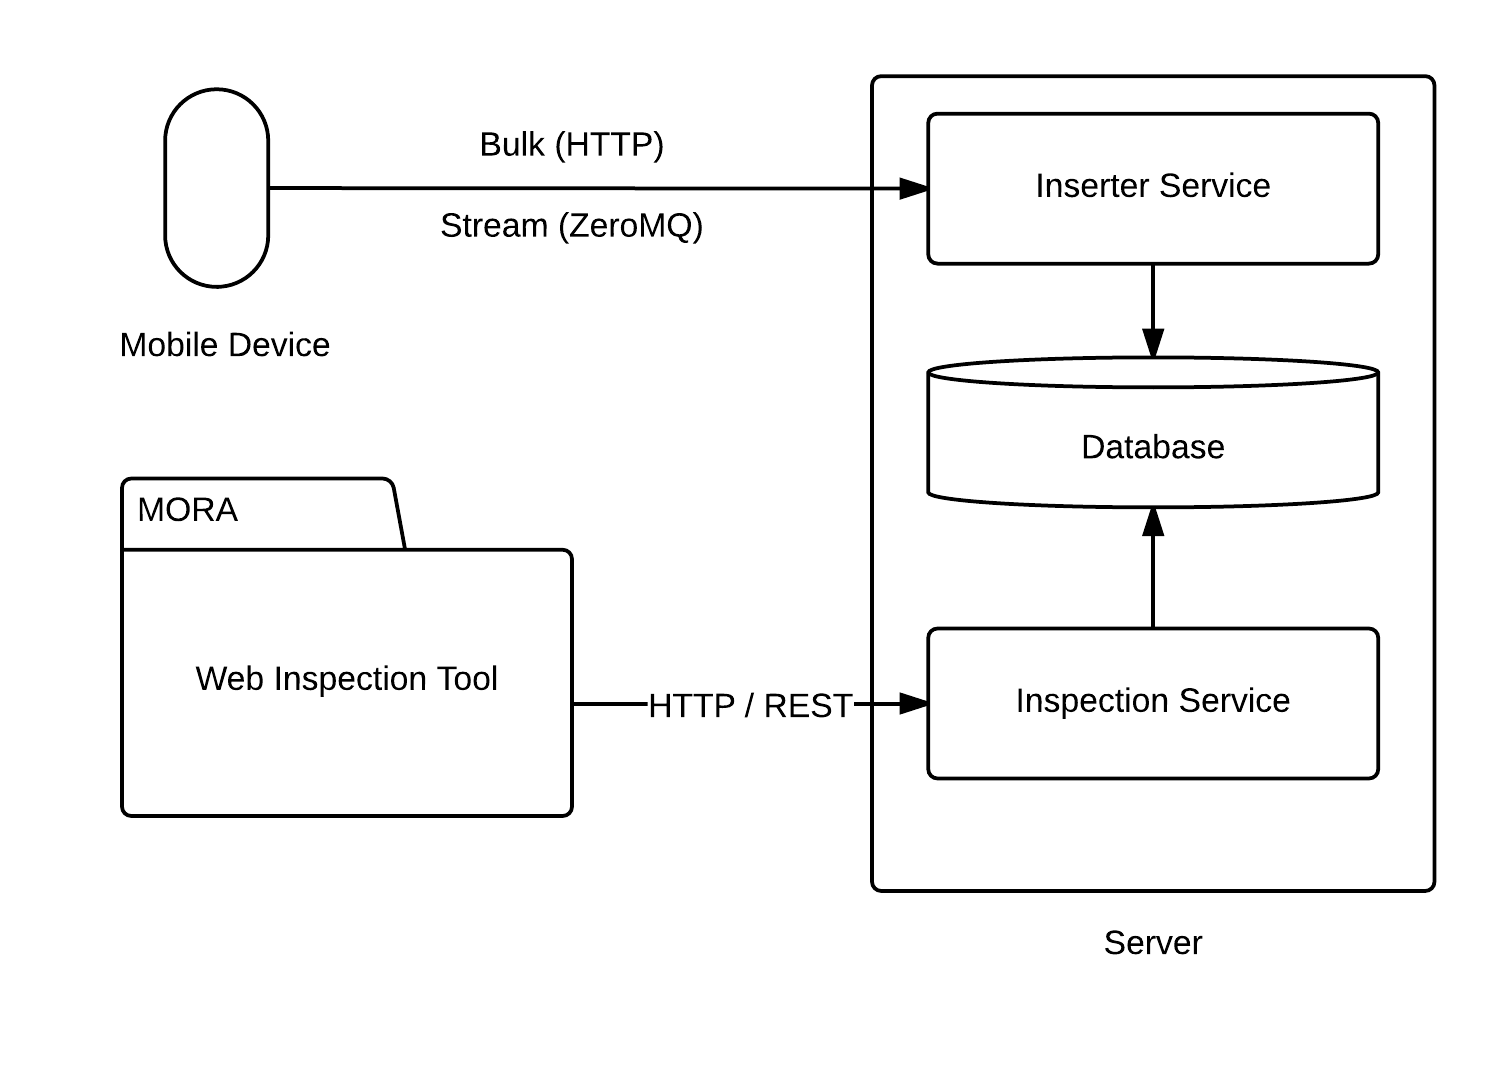
\includegraphics[width=\linewidth]{img/system_overview.png}
\caption{MORA System Overview}
\label{overview}
\end{figure}

\SubSection{Mobile Sensor Collector}

* Figure: new GUI from Lukas

* Goals and 'Requirements'
  - Correctness of data / good performance
  - View sensor data as events, that are logged / streamed / processed
  - Extensible by analysis plugins
  - Transfer of sensor data to server

* Service + Example GUI (Communication with Intent bindings)
  - Android lifecycle forces collector to be a service
  - Standalone use of service possible and intended

* Available Sensors. Types of sensors. Class Hierarchy.

* Data flow from Sensor Event to Log file,
  in analogy to logging frameworks.
  Use of Threads

* Transfer via HTTP and Streaming

* Configuration options with configuration file and GUI

* Log messages are written to a file

* Extendability with Plugins: Consumer/Producer. Examples:
  - HAR
  - GPS Cache
  - Intent producer

\SubSection{Sensor Storage Server}

* HTTP server (tomcat/Node), that accepts POST request

* Stores in FS and in DB

* Sends 200 Status code if insert in db complete

* JSF Data Exchange Format

* Auto Creation of DB Tables for new sample types (JSON data type)

\SubSection{Web Inspection Tool}
\url{liveandgov.uni-koblenz.de/storage/inspection}

+ Figure: Screenshot mit Bar-Code Anzeige von Activities

* Purpose: View on DB tables for inspection of raw data
  and results of data mining.
  - Which recordings have made it to the db? Transfer successful?
  - Rough measure for Quality of recorded data. Constant frequency? Accuracy of GPS? can be judged from plots.
  - Simple export of sample bulks as CSV for processing with other applications.
  - Inspection of data mining results.
  - Privacy Aspects. Give users control over the data.

* Features:
  - Browser based
  - Zoom
  - Views:
    - Plots of time series data (e.g. accelerometer)
    - Map based views of GPS data
    - Lists of textual data (tags)
    - Bar-Code-like view of Tags
    - Map markers of tags
  - Delete recordings
  - Automatic display of available tables
    -> as text (TEXT) or plot (float)

* Mining output has to be stored in db
  - Can be created on mobile device and inserted into transfer file
  - Or can be done on the server

%-------------------------------------------------------------------------
\Section{Practical Examples}

\SubSection{Human Activity Recognition}
* Decision tree learning with WEKA
* Import classifier as JAVA class into MORA Library

\SubSection{Service Line Detection}
* Web service for SLD
* GPS Samples are gathered via MORA lib
* Query results are inserted back into MORA
* Analysis of classification results via inspection tool

%-------------------------------------------------------------------------
\Section{Related Work}

* FUNF
* SDCF


\nocite{ex1,ex2}
\bibliographystyle{latex8}
\bibliography{latex8}

\end{document}
